\documentclass[10pt]{article}

\usepackage[letterpaper,top=0.56in,bottom=0.55in,left=0.65in,right=0.65in]{geometry}
\usepackage{booktabs}
\usepackage{enumitem}
\usepackage{hyperref}
\usepackage{microtype}
\usepackage{multicol}
\usepackage{tabularx}
\usepackage{tikz}
\usepackage{titlesec}
\usepackage{xcolor}
\usetikzlibrary{arrows.meta,positioning}

\definecolor{kept}{HTML}{E8F5E9}
\definecolor{redo}{HTML}{E8EAFB}
\definecolor{fault}{HTML}{FDEBEC}
\definecolor{softgray}{HTML}{F3F3F3}
\definecolor{linkblue}{HTML}{006D8F}

\hypersetup{colorlinks=true,urlcolor=linkblue,linkcolor=black}
\setlength{\columnsep}{0.30in}
\setlength{\parindent}{1em}
\setlength{\parskip}{0pt}
\setlist[itemize]{leftmargin=1.15em,itemsep=1pt,topsep=2pt}
\titleformat{\section}{\centering\bfseries\large}{}{0pt}{}
\titlespacing*{\section}{0pt}{6pt}{3pt}
\pagestyle{plain}

\begin{document}

\begin{center}
    {\LARGE\bfseries Selective Recovery for Cascading Failures\\[-1pt]
    in Multi-Agent LLM Systems\par}
    \vspace{7pt}
    Lucas Yan \quad Atharv Nair \quad Utkarsh Ranjan \quad Ethan Chen \quad Bijin Kurian Jiby

    \vspace{5pt}
    CSE 291A Phase 1 Report (Option 5: Failure Propagation and Recovery in Multi-Agent Systems)
\end{center}

\vspace{2pt}
\begin{multicols}{2}
\small

\section*{Problem}

Multi-agent workflows can fail after completing useful work or causing external side effects. A full restart recomputes every stage, discards valid work, and cannot by itself undo irreversible effects such as sent email. We study recovery after the faulty step is already known: which dependent work must be redone, which work can be reused, and which effects must be undone, compensated, or only reported?

Our current system is a travel-booking pipeline with flight and hotel research stages, a planner, and an executor. Every step records artifacts, dependencies, tool calls, and side effects in a provenance graph. Recovery methods begin from the same faulty world rather than receiving a free reset.

\section*{Phase 1 Question}

\begin{center}
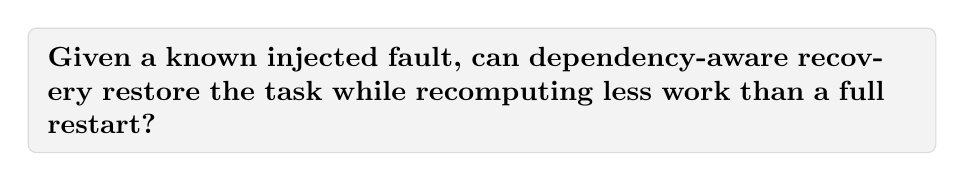
\begin{tikzpicture}
\node[
    draw=black!14, fill=softgray, rounded corners=3pt,
    inner sep=7pt, text width=0.91\columnwidth, align=left
] {\bfseries Given a known injected fault, can dependency-aware recovery restore the task while recomputing less work than a full restart?};
\end{tikzpicture}
\end{center}

\section*{System and Recovery}

The seeded generator creates tasks with exact flight, hotel, constraint, and email ground truth. Ten faults cover observations, agent outputs, plans, tool selection, tool arguments, and one malicious instruction. We compare full restart, suffix replay, coarse lineage, support lineage, monitor, support-monitor, and always-verify. Coarse lineage follows all recorded context dependencies; support lineage follows evidence actually cited by later steps.

\begin{center}
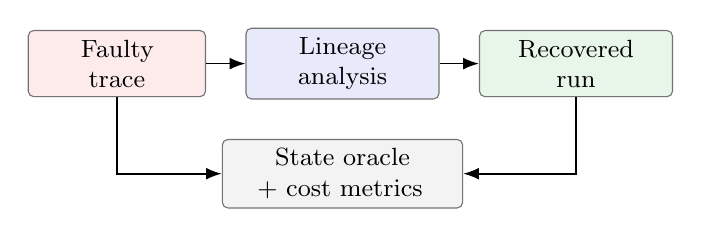
\begin{tikzpicture}[
    node distance=4mm and 5mm,
    box/.style={draw=black!55, rounded corners=2pt, minimum height=7mm,
                align=center, font=\small, inner xsep=5pt},
    arrow/.style={-{Latex[length=2mm]}, semithick}
]
\node[box, fill=fault, text width=19mm] (fault) {Faulty\\trace};
\node[box, fill=redo, text width=21mm, right=of fault] (prov) {Lineage\\analysis};
\node[box, fill=kept, text width=21mm, right=of prov] (recover) {Recovered\\run};
\draw[arrow] (fault) -- (prov);
\draw[arrow] (prov) -- (recover);
\node[box, fill=softgray, text width=27mm, below=5mm of prov] (oracle) {State oracle\\+ cost metrics};
\draw[arrow] (fault.south) |- (oracle.west);
\draw[arrow] (recover.south) |- (oracle.east);
\end{tikzpicture}

\small Figure 1: Paired evaluation from one shared faulty execution. Red is the trace, blue is lineage analysis, and green is the recovered run.
\end{center}

\section*{Evaluation Design}

Five primary metrics answer correctness and cost:
\begin{itemize}
    \item task recovery success;
    \item recovery side-effect integrity;
    \item token ratio relative to restart;
    \item latency ratio relative to restart; and
    \item valid-work preservation.
\end{itemize}
Final-effect integrity, irreversible harm, and global/recovery unauthorized-action rates are reported separately. This prevents damage already caused by the faulty run from being mislabeled as a recovery failure.

\columnbreak

\section*{Benchmarks and Data}

The internal paired harness is the main benchmark because it directly matches our assumption that fault location is known. \href{https://github.com/tradertanmay/undobench}{\textbf{UndoBench}} adds operational tasks with state and side-effect oracles. Our adapter retries a known pre-mutation failure once; it does not recover a trajectory after a committed effect. \href{https://github.com/SaFo-Lab/A2ASecBench}{\textbf{A2ASecBench}} adds matched attack/control cases for agent-to-agent protocols. Its adapter measures tainted-action blocking, not rollback after effects occur.

We also reviewed \href{https://github.com/microsoft/TAMAS}{\textbf{TAMAS}} and \href{https://huggingface.co/datasets/Kevin355/Who_and_When}{\textbf{Who\&When}}. TAMAS requires a paid model API, so it is excluded from Phase 1 numbers without approval. Who\&When traces are useful for attribution analysis but are not executable recovery environments for this workflow.

\section*{Quantitative Progress}

\footnotesize
\begin{tabularx}{\columnwidth}{@{}>{\raggedright\arraybackslash}X >{\raggedleft\arraybackslash}p{0.18\columnwidth} >{\raggedleft\arraybackslash}p{0.38\columnwidth}@{}}
\toprule
\textbf{Evidence} & \textbf{Scale} & \textbf{Observed result} \\
\midrule
Automated suite & 64 tests & 64 passed \\
Internal harness & 10 faults & mock: all fire; plumbing only \\
UndoBench smoke & 4 pairs & 4 controls; 2 recovered \\
A2ASecBench & 800 records & attack success rate 0; control pass 1.0 \\
\bottomrule
\end{tabularx}
\small

UndoBench's recovery rate is 0.50 with zero duplicate effects in the four-pair smoke suite. A2ASecBench covers ASRF, ATSI, coordination oscillation, and task flooding (200 records each; one trial per suite). Its perfect preliminary score is policy-specific: the task-flooding adapter uses a declared five-task quota and still needs a sensitivity sweep.

\section*{Phase 1 Status}

\textbf{The repository meets the Phase 1 requirement.} It contains a reproducible dataset generator, ten fault injections, explicit oracles and metrics, seven recovery/prevention methods, two executable external adapters, machine-readable result rows, provenance traces, and 64 passing tests.

\textbf{The final empirical claim is not complete.} Phase 2 must run the fixed local Qwen2.5-7B model on 30 seeds, 10 faults, and six recovery methods (1,800 paired comparisons), retain failures and timeouts, repeat runs for confidence intervals, evaluate held-out seeds, and sweep the task-flooding quota. Mock-LLM and unapproved paid-API outputs will not be reported as results.

\end{multicols}

\clearpage
\appendix
\section*{Appendix A: Timeline and Milestones}

\renewcommand{\arraystretch}{1.12}
\begin{tabularx}{\textwidth}{@{}>{\raggedright\arraybackslash}p{0.19\textwidth} >{\raggedright\arraybackslash}X >{\raggedright\arraybackslash}p{0.17\textwidth}@{}}
\toprule
\textbf{Period} & \textbf{Milestone and deliverable} & \textbf{Exit criterion} \\
\midrule
Phase 1: Harness &
Seeded multi-agent workflow, provenance graph, effect classes, deterministic world oracle, and ten fault injections. &
\textbf{Complete} \\

Phase 1: Evaluation &
Five primary metrics; separate final/recovery effects and irreversible harm; JSONL summaries and trace artifacts. &
\textbf{Complete} \\

Phase 1: External validation &
Native UndoBench and A2ASecBench adapters, automated regression tests, and reproduced smoke results. &
\textbf{Complete} \\

Phase 2, Week 1 &
Measure local-model clean-run reliability and determinism; freeze model, prompts, temperature, seeds, and schedules. &
Reliable clean baseline \\

Phase 2, Week 2 &
Run 30 seeds $\times$ 10 faults $\times$ 6 recovery methods; retain failures and compute paired token/latency ratios. &
1,800 paired trials \\

Phase 2, Week 3 &
Repeat runs, calculate confidence intervals, evaluate held-out seeds, and sweep task quotas (1, 5, 10, 20). &
Stable estimates \\

Final phase &
Analyze failure cases and ablations; verify claims against artifacts; produce final tables, report, and presentation. &
Submission package \\
\bottomrule
\end{tabularx}

\section*{Appendix B: Reproducibility}

\begin{multicols}{2}
\small
\textbf{Main paired experiment}
\begin{verbatim}
uv sync
uv run pytest -q
# In a separate terminal:
./scripts/start_server.sh
# Back in this terminal:
uv run agentrec experiment \
  --tasks 30 --faults all \
  --methods restart,suffix,coarse,\
support,monitor,support_monitor
uv run python analysis/summarize.py \
  results/experiment-server-*/rows.jsonl
\end{verbatim}

\columnbreak
\textbf{External benchmark smoke tests}
\begin{verbatim}
uv run agentrec undobench download
uv pip install -e data/undobench-upstream
uv run agentrec undobench trial \
  --suite smoke --recovery agentrec

uv run agentrec a2a download
uv pip install -e \
  'data/a2asec-upstream[dev]'
for s in asrf atsi co hotf; do
  uv run agentrec a2a trial \
    --config configs/offline/${s}_eval.yaml \
    --agentrec
done
\end{verbatim}
\end{multicols}

\end{document}
